\documentclass[aspectratio=169]{beamer}

% SETUP =====================================
\usepackage[T1,T2A]{fontenc}
\usepackage[utf8]{inputenc}
\usepackage[russian]{babel}
\usepackage{listings}
\usepackage{array}
\usepackage{amssymb}
\usepackage{pifont}
\usepackage{minted}
\usepackage{../../beamerthemeslidesgeneric}
% SETUP =====================================

\title{Scala Typesystem II}
\author{Mikhail Mutcianko, Alexey Shcherbakov}
\institute{СПБгУ, СП}
\date{25 февраля 2021}

\begin{document}

\frame{\titlepage}

\section{Syntax recap: Advaned Features}

% multi parens and currying
\begin{frame}[fragile]{Parameter lists}
\begin{lstlisting}[style=scala]
def foldLeft[B](z: B)(op: (B, A) => B): B
\end{lstlisting}
\begin{itemize}
  \item logical grouping
  \item partial application
  \item passing implicit arguments
  \item assisting the typechecker
\end{itemize}
\end{frame}

\begin{frame}[fragile]{Type inference of multi-paren}
  \begin{block}{}
    Types are inferred sequentially per \alert{each complete} parenthesis
  \end{block}
  \vspace{2em}
\begin{lstlisting}[style=scala]
def foo[A](x: A, f: A => Int) = ???
~def bar[A](x: A)(f: A => Int) = ???~

object Demo {
  foo(1, i => i * i) // <<< error: missing parameter type
  ~bar(2)(i => i * i)~
}~~
\end{lstlisting}
\end{frame}

% named and default parameters
\begin{frame}[fragile]{Named parameters}
\begin{itemize}
  \item arguments could be labelled with their parameter names
  \item order of named arguments can be rearranged
  \item the unnamed arguments must come first
\end{itemize}
\pause
\vspace{2em}
\begin{lstlisting}[style=scala]
||def printName(first: String, last: String) = ???

printName("John", "Smith")                     // Prints "John Smith"
printName(first = "John", last = "Smith")  // Prints "John Smith"
printName(last = "Smith", first = "John")  // Prints "John Smith"
printName(last = "Smith", "john")              // <<< error: positional after named argument
\end{lstlisting}
\end{frame}

% call by name parameters
  % example: custom control structures
\begin{frame}{Call by-name parameters}
\begin{block}{}
By-name parameters are only evaluated when used. They are in contrast to by-value parameters. To
make a parameter called by-name, simply prepend \texttt{=>} to its type.
\end{block}
\begin{itemize}
  \item evaluated at \alert{each} use within the function
  \item not the same thing as function-typed parameter
  \item can be used to pass blocks of code
\end{itemize}
\end{frame}

\begin{frame}[fragile]{Call by-name parameters}{Example}
\begin{lstlisting}[style=scala]
p: () => Boolean    // a function input parameter
p: => Boolean       // a by-name parameter

~myAssert(() => 5 > 3)~
~byNameAssert(5 > 3)~
\end{lstlisting}
\pause
\begin{lstlisting}[style=scala]
def whileLoop(condition: => Boolean)(body: => Unit): Unit =
  if (condition) {
    body
    whileLoop(condition)(body)
  }

whileLoop (i > 0) {
  println(i)
  i -= 1
}
\end{lstlisting}
\end{frame}

% type aliases
\begin{frame}[fragile]{Type aliases}
\begin{block}{}
  A type alias creates a new named type for a specific, existing type
\end{block}
\vspace{1em}
\begin{lstlisting}[style=scala]
type Word = List[Char]
type Sentence = List[Word]
type Paragraph = List[Sentence]
\end{lstlisting}
\pause
Poor practice example:
\begin{lstlisting}[style=scala]
type IntMaker = () => Int
IntMaker
\end{lstlisting}
\end{frame}

\section{Advanced OOP}

\begin{frame}{Final keyword}
  In Scala \texttt{final} keyword is used to restrict inheritance
  \begin{itemize}
    \item final val/var/def - prohibits overriding
    \item final class - prohibits inheritance
  \end{itemize}
\end{frame}

\begin{frame}{Linearization}
\begin{block}{}
  Scala \texttt{linearization}\cite{spec-lin} is a deterministic process that puts all traits in a linear inheritance
  hierarchy
\end{block}
\pause
\begin{enumerate}
  \item start at the first extended class or trait and write that complete hierarchy down
  \item take the next trait and write this hierarchy down
    \begin{itemize}
      \item  remove all classes/traits from this hierarchy which are already in the linearized
        hierarchy
      \item add the remaining traits to the bottom of the linearized hierarchy to create the new
        linearized hierarchy
    \end{itemize}
    \item repeat step 2 for every trait
    \item place the class itself as the last type extending the linearized hierarchy
\end{enumerate}
\end{frame}

% linearization
\begin{frame}[fragile]{Linearization}
  \begin{columns}
    \begin{column}{0.5\textwidth}
      \begin{onlyenv}<2->
        \begin{center}
          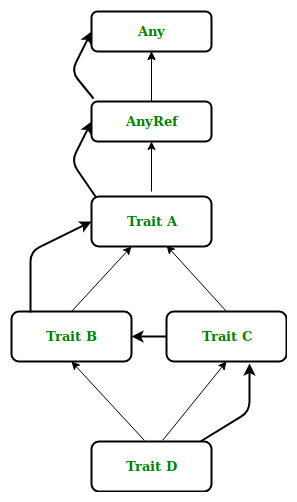
\includegraphics[scale=0.3]{linear}
        \end{center}
        \hrule\vspace{3pt}
        \noindent\tiny bold --- \texttt{Linearization} \\ \vspace{-1em}
        \noindent\tiny light --- \texttt{Inheritance}
      \end{onlyenv}
    \end{column}
    \begin{column}{0.5\textwidth}
      \begin{onlyenv}<1->
        \begin{lstlisting}[style=scala]
trait A
trait B extends A
trait C extends A
class D extends B with C
        \end{lstlisting} 
      \end{onlyenv} 
      \vspace{2em}
      \begin{onlyenv}<3->
        Actual hierarchy: \\
        \texttt{D $\rightarrow$ C $\rightarrow$ B $\rightarrow$ A $\rightarrow$ AnyRef $\rightarrow$ Any}
      \end{onlyenv}
    \end{column}
  \end{columns}
\end{frame}

% abstract overrides
\begin{frame}[fragile]{Abstract overrides}
  Scala allows invoking an abstract method of a superclass
\begin{itemize}
  \item the meaning of super is not known at compile time in a single trait
  \item \texttt{super} calls in a trait are dynamically bound via linearization
  \item trait methods that need to call \texttt{super} must be annotated with \texttt{abstract
    override}
\end{itemize}
\end{frame}

\begin{frame}[fragile]{Abstract overrides}{Example}
\begin{minted}{scala}
trait IntPrinter
  { def print(a: Int) }
class PrinterImpl extends IntPrinter
  { def print(a: Int) = println(a) }
trait DoublingPrinter extends IntPrinter
  { abstract override def print(a: Int) = super.print(a*2) }

|\pause|(new PrinterImpl).print(3)                      // prints 3
|\pause|(new PrinterImpl with DoublingPrinter).print(3) // prints 6
\end{minted}
\end{frame}

% self type
\begin{frame}[fragile]{Self type}
\begin{block}{}
Self-types are a way to declare that a trait must be mixed into another trait, even though it
doesn’t directly extend it. That makes the members of the dependency available without imports
\end{block}
\vspace{2em}
\pause
\begin{minted}{scala}
trait Defns { this: Aggregate => ...}
trait Utils { this: Aggregate => ...}

object Aggregate extends Defns with Utils with ...
\end{minted}
\end{frame}

 %path dependent types
\begin{frame}[fragile]{Path dependent types}
  \vspace{-1em}
  \begin{block}{}
    In Scala, a nested type is bound to a specific \alert{instance}  of the outer type, not to the outer type
    itself
  \end{block}
  \begin{onlyenv}<2>
    \begin{minted}{scala}
      class Foo {
        class Bar
        var bar: Bar = new Bar
      }
      val a = new Foo
      val b = new Foo
      a.bar = b.bar //error: type mismatch; found: b.Bar; required: a.Bar
    \end{minted}
  \end{onlyenv}
  \begin{onlyenv}<3>
    \hig{3,7}
    \begin{minted}{scala}
      class Foo {
        class Bar
        var bar: Foo#Bar = new Bar
      }
      val a = new Foo
      val b = new Foo
      a.bar = b.bar // OK
    \end{minted}
  \end{onlyenv}
\end{frame}

\begin{frame}[fragile]{Path dependent types}{Muli-paren}
\begin{minted}{scala}
case class Animal(foodName: String) { 
  case class Food(name: String)
  val food = Food(foodName)
}

def feed(animal: Animal)(food: animal.Food) = ???

val cat = Animal("fish")
val fish = Animal("seaweed")
feed(cat)(fish.food) // error: found: fish.Food, required: cat.Food
\end{minted}
\end{frame}

% compound types
\begin{frame}{Compound types}
  \begin{itemize}
    \item express that the type of an object is a subtype of several other types
    \item resulting type is an intersections of object types
    \item the general form is: \mintinline{scala} |A with B with C ... { refinement }|
  \end{itemize}
\end{frame}

\begin{frame}[fragile]{Compound types}
\hig{4}
\begin{minted}{scala}
trait Str { def str: String }
trait Count { def count: Int }

def repeat(cd: Str with Count): String =
  Iterator.fill(cd.count)(cd.str).mkString

repeat(new Str with Count {
  val str = "test"
  val count = 3
}) // "testtesttest"
\end{minted}
\end{frame}

\section{Polymorphic Types}

% OOP polymorphism
\begin{frame}[fragile]{Subtype polymorphism}
  \vspace{-2em}
\begin{block}{}
  Subclasses of a class can define their own unique behaviors while providing a common access
  interface. Instances of a subclass can be passed to a base class
\end{block}
\begin{minted}{scala}
trait Animal { def speak }
class Human extends Animal { def speak = println("foo") }

val animal: Animal = new Human
animal.speak
\end{minted}
\end{frame}

% type parameters
\begin{frame}[fragile]{Type parameters}
  Allow abstracting over types in a class or a method
  \begin{itemize}
    \item class parameters are bound on \alert{construction}
    \item method parameters are bound on \alert{invocation} 
  \end{itemize}
  \vspace{1em}
  \pause
  \begin{onlyenv}<2>
    %\hig{7}
    \begin{minted}{scala}
      class A[T] {
        def foo(t: T) = ???
      }

      val a = new Foo[Int]
      a.foo(123)    // OK
      a.foo("123")  // compile error: found: String, required: Int
    \end{minted}
  \end{onlyenv}
  \begin{onlyenv}<3>
    \hig{2,7}
    \begin{minted}{scala}
      class A {
        def foo[T](t: T) = ???
      }

      val a = new Foo[Int]
      a.foo(123)    // OK
      a.foo("123")  // OK
    \end{minted}
  \end{onlyenv}
\end{frame}


% pattern matching and erasure
\begin{frame}{Type erasure}
\begin{block}{Scalac warning:}
\ttfamily non-variable type argument Int in type pattern Seq[Int] (the underlying
of Seq[Int]) is unchecked since it is eliminated by erasure
\end{block}
\vspace{2em}
\pause
\begin{block}{Type parameters do not affect evaluation in Scala}
  We can assume that all type parameters and type arguments are removed before evaluating the
  program
\end{block}
\end{frame}

\begin{frame}[fragile]{Type erasure}
\only<2>{\hig{4,9}}
\begin{minted}{scala}
def process(thing: SomeThing[_]) = thing match {
  case _: Int         => "an int"
  case _: Seq[Int]    => "some ints"
  case _: Seq[String] => "some strings"
}

process(123) == "an int"
process(Seq(1,2,3)) == "some ints"
process(Seq("1", "2", "3")) == "some ints"
\end{minted}
\end{frame}

% subtyping relations
\begin{frame}{Type bounds}
\vspace{-2em}
\begin{block}{}
   Type bounds limit the concrete values of the type variables and possibly reveal \alert{more} information
   about the members of such types
\end{block}
\begin{itemize}
  \item \texttt{A <: B} means: \texttt{A} is a subtype of \texttt{B}
  \item \texttt{A >: B} means: \texttt{A} is a supertype of \texttt{B}, or \texttt{B} is a subtype
    of \texttt{A}
\end{itemize}
\end{frame}

\begin{frame}[fragile]{Type bounds}{Upper bounds}
\hig{7}
\begin{minted}{scala}
trait Animal                 { def fitness: Int }
trait Reptile extends Animal
trait Mammal  extends Animal
trait Zebra   extends Mammal { def zebraCount: Int }
trait Giraffe extends Mammal

def selection[A <: Animal](a1: A, a2: A): A =
  if (a1.fitness > a2.fitness) a1 else a2
\end{minted}
\end{frame}

\begin{frame}[fragile]{Type bounds}{Lower and mixed bounds}
  \begin{minted}{scala}
  def reptilize[A >: Reptile](stuff: A): A = ???
  \end{minted}
  \begin{itemize}
    \item the type parameter \texttt{A} that can range only over \alert{supertypes}  of \texttt{Reptile}
    \item \texttt{A} could be one of \texttt{Reptile}, \texttt{Animal}, \texttt{AnyRef} or \texttt{Any}
  \end{itemize}
  \vspace{3em}
  \pause
  \begin{minted}{scala}
  def hide[A >: Zebra <: Animal](stuff: A): A = ???
  \end{minted}
  \begin{itemize}
    \item restrict \texttt{A} any type on the interval between \texttt{Zebra} and \texttt{Animal}
  \end{itemize}
\end{frame}

% variance
\begin{frame}[fragile]{Variance}
  \vspace{-2em}
  \begin{block}{}
  Variance is the correlation of subtyping relationships of complex types and the subtyping
  relationships of their component types
  \end{block}
  \vspace{-1em}
  \begin{block}{}
    Scala supports variance annotations of type parameters of \alert{generic classes}
  \end{block}
  \vspace{1em}
  \begin{minted}{scala}
  class Foo[+A] // A covariant class
  class Bar[-A] // A contravariant class
  class Baz[A]  // An invariant class
  \end{minted}
\end{frame}

\begin{frame}[fragile]{Covariance}
  \begin{block}{}
  Let \texttt{C[T]} be a parameterized type and \texttt{A}, \texttt{B} are types such that \texttt{A <:
  B} \\
  and if \texttt{C[A] <: C[B]} then \texttt{C} is \alert{covariant} 
  \end{block}
  \vspace{1em}
\begin{onlyenv}<1>
    \begin{minted}{scala}
  class Foo[A] { def f(x: Foo[A]) = ??? }

  val foo = new Foo[Number]
  foo.f(new Foo[Int]) // error: type mismatch found: Foo[Int], required: Foo[Number]
  \end{minted}
\end{onlyenv}
\begin{onlyenv}<2>
  \hig{1,4}
    \begin{minted}{scala}
  class Foo[+A] { def f[T <: A](x: Foo[T]) = ??? }

  val foo = new Foo[Number]
  foo.f(new Foo[Int]) // OK
  \end{minted}
\end{onlyenv}
\end{frame}

% sidenote: variance of java arrays
\begin{frame}[fragile]{Java array variace}
  Early version of Java had no generics but polymorphic array algorithms were still necessary:
  \vspace{1em}
  \begin{minted}{java}
  boolean equalArrays (Object[] a1, Object[] a2);
  void shuffleArray(Object[] a);
  \end{minted}
  \vspace{1em}
  \pause
  \begin{minted}{java}
Zebra[] zebras = new Zebra[]{ new Zebra() }  // Array containing 1 `Zebra`
Mammal[] mammals = zebras  // Allowed because arrays are covariant in Java
mammals[0] = new Giraffe() // Allowed because a `Giraffe` is a subtype of `Mammal`
Zebra zebra = zebras[0]    // Get the first `Zebra` … which is actually a `Giraffe`!
  \end{minted}
\end{frame}

\begin{frame}[fragile]{Java array variance}{ArrayStoreException}
  To mitigate invalid array type storage issue Java has introduced
  \texttt{ArrayStoreException} \cite{arstex}
  \vspace{3em}
  \begin{minted}{java}
     Object x[] = new String[3];
     x[0] = new Integer(0); // ArrayStoreException is thrown
  \end{minted}
\end{frame}

% var overriding
\begin{frame}[fragile]{var overriding}
\begin{block}{Question}
  Why can't you override a var?
\end{block}
\pause
\begin{minted}{scala}
class Foo {          var animal: Animal }
class Bar { override var animal: Cat    } extends Foo

val bar: Bar      = new Bar
val barAsFoo: Foo = bar
barAsFoo.animal   = new Dog
bar.animal // <<< ???
\end{minted}
\end{frame}

% scala immutable collections are covariant - mutable invariant
\begin{frame}[fragile]{Scala collections variance}
  %\vspace{-2em}
\begin{itemize}
  \item \texttt{immutable} Scala collections are \alert{covariant}
  \item \texttt{mutable} Scala collections are \alert{invariant}
  \item \texttt{Array} in Scala is \alert{invariant}
\end{itemize}
\begin{onlyenv}<2>
  \vspace{2em}
\begin{minted}{scala}
val zebras: Array[Zebra] = Array(new Zebra)
val mammals: Array[Mammal] = zebras //error: found: Array[Zebra], required: Array[Mammal]
mammals(0) = new Giraffe
val zebra: Zebra = zebras(0)
\end{minted}
\end{onlyenv}
\begin{onlyenv}<3>
  \vspace{2em}
\begin{minted}{scala}
val zebras: List[Zebra] = List(new Zebra)
val mammals: List[Mammal] = zebras
val something = mammals :+ new Giraffe
val zebra: Zebra = zebras.tail.head // OK
\end{minted}
\end{onlyenv}
\end{frame}

% variance for functions
\begin{frame}[fragile]{Scala function variance}
\vspace{-2em}
\begin{block}{}
If \texttt{A2 <: A1} and \texttt{B1 <: B2} then \texttt{A1 => B1 <: A2 => B2} \\
So functions are contravariant in argument type(s) and covariant in result type
\end{block}
\vspace{1em}
\begin{minted}{scala}
trait Function1[-T, +U] {
  def apply(x: T): U
}
\end{minted}
\pause
\vspace{1em}
\begin{minted}{scala}
  class Foo[+A] { def f(x: Foo[A]) = ??? }
  //                    ^
  // error: covariant type A occurs in contravariant position in type Foo[A] of value x
\end{minted}
\end{frame}


\begin{frame}[fragile]{Variance checks}
The Scala compiler will check that there are no problematic combinations when compiling a class with
variance annotations. Roughly:
\begin{itemize}
  \item covariant type parameters can only appear in method results
  \item contravariant type parameters can only appear in method parameters
  \item invariant type parameters can appear anywhere
    \pause
  \item covariant type parameters may appear in lower bounds of method type parameters
  \item contravariant type parameters may appear in upper bounds of method
\end{itemize}
\end{frame}

% abstract type members
\begin{frame}[fragile]{Type members}
  Abstract types, such as traits and abstract classes, can in turn have abstract type members. This
  means that the concrete implementations define the actual types.
  %\vspace{1em}
  \begin{onlyenv}<1>
      \hig{9}
      \begin{minted}{scala}
    trait Buffer {
      type T
      val element: T
      def copyFrom(t: T)
    }
    abstract class SeqBuffer extends Buffer {
      type U
      type T <: Seq[U]
      def length = element.length
    }
      \end{minted}
  \end{onlyenv}
  \begin{onlyenv}<2>
      \hig{7,9}
      \begin{minted}{scala}
    trait Buffer {
      type T
      val element: T
      def copyFrom(t: T)
    }
    class IntSeqBuffer extends Buffer {
      override type T = Seq[Int]
      def length = element.length
      def copyFrom(t: Seq[Int]) = ???
    }
      \end{minted}
  \end{onlyenv}
\end{frame}

% structural types & refined types
% this(singleton) types
% F-bound types
% existential types
% higher kinded types
% partial application of HKT and kind-projector plugin


\begin{thebibliography}{9}
  \bibitem{spec-lin}
  \url{https://www.scala-lang.org/files/archive/spec/2.11/05-classes-and-objects.html#class-linearization}
  \bibitem{fpdt}
  \url{http://lampwww.epfl.ch/~amin/dot/fpdt.pdf}
  \bibitem{miles-pdt}
  \url{https://stackoverflow.com/questions/12935731/any-reason-why-scala-does-not-explicitly-support-dependent-types/12937819#12937819}
  \bibitem{arstex}
  \url{https://docs.oracle.com/javase/7/docs/api/java/lang/ArrayStoreException.html}
\end{thebibliography}

\end{document}

